\begin{figure}[t]
  \centering
  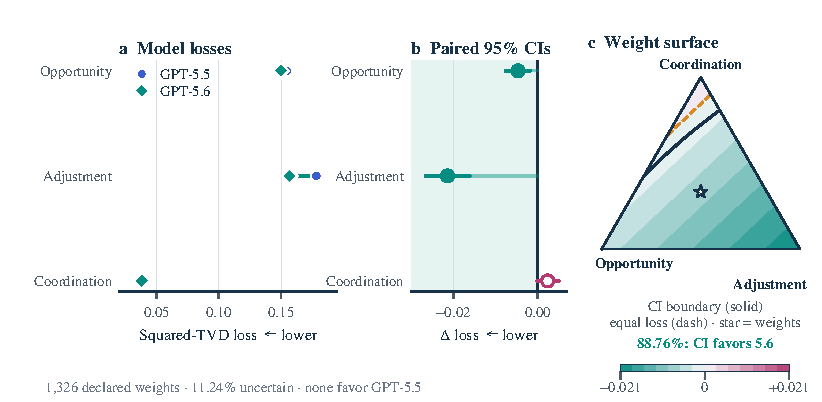
\includegraphics[width=\linewidth]{figs/fig3_economic_story.pdf}
  \caption{Theory-indexed economic sensitivity; negative contrasts favor GPT-5.6.
  \textbf{a}, Connected dumbbells compare model-specific mean squared-TVD loss for the
  three declared margins. \textbf{b}, Lollipops give paired country-bootstrap 95\% BCa intervals; fill
  marks the three-margin Holm results. \textbf{c}, a continuous surface over all 1,326
  nonnegative 0.02-grid weight vectors. Fill encodes $\Delta$ weighted loss; the solid
  line is the upper-95\%-CI zero boundary, the dashed line equal point loss, and the star
  equal weights. Fully named vertices prevent the area from being mistaken for a fourth
  outcome. The grid is one descriptive sensitivity analysis, not 1,326 separately
  corrected tests. These are representation losses under declared weights, not welfare
  or policy-effect estimates.}
  \label{fig:economic-story}
\end{figure}
